\documentclass[conference, onecolumn]{IEEEtran}

% *** GRAPHICS RELATED PACKAGES ***
%
\ifCLASSINFOpdf
  \usepackage[pdftex]{graphicx}
  % declare the path(s) where your graphic files are
  % \graphicspath{{../pdf/}{../jpeg/}}
  % and their extensions so you won't have to specify these with
  % every instance of \includegraphics
  % \DeclareGraphicsExtensions{.pdf,.jpeg,.png}
\else
  % or other class option (dvipsone, dvipdf, if not using dvips). graphicx
  % will default to the driver specified in the system graphics.cfg if no
  % driver is specified.
  % \usepackage[dvips]{graphicx}
  % declare the path(s) where your graphic files are
  % \graphicspath{{../eps/}}
  % and their extensions so you won't have to specify these with
  % every instance of \includegraphics
  % \DeclareGraphicsExtensions{.eps}
\fi
% graphicx was written by David Carlisle and Sebastian Rahtz. It is
% required if you want graphics, photos, etc. graphicx.sty is already
% installed on most LaTeX systems. The latest version and documentation can
% be obtained at: 
% http://www.ctan.org/tex-archive/macros/latex/required/graphics/
% Another good source of documentation is "Using Imported Graphics in
% LaTeX2e" by Keith Reckdahl which can be found as epslatex.ps or
% epslatex.pdf at: http://www.ctan.org/tex-archive/info/
%
% latex, and pdflatex in dvi mode, support graphics in encapsulated
% postscript (.eps) format. pdflatex in pdf mode supports graphics
% in .pdf, .jpeg, .png and .mps (metapost) formats. Users should ensure
% that all non-photo figures use a vector format (.eps, .pdf, .mps) and
% not a bitmapped formats (.jpeg, .png). IEEE frowns on bitmapped formats
% which can result in "jaggedy"/blurry rendering of lines and letters as
% well as large increases in file sizes.
%
% You can find documentation about the pdfTeX application at:
% http://www.tug.org/applications/pdftex





% *** MATH PACKAGES ***
%
\usepackage[cmex10]{amsmath}
% A popular package from the American Mathematical Society that provides
% many useful and powerful commands for dealing with mathematics. If using
% it, be sure to load this package with the cmex10 option to ensure that
% only type 1 fonts will utilized at all point sizes. Without this option,
% it is possible that some math symbols, particularly those within
% footnotes, will be rendered in bitmap form which will result in a
% document that can not be IEEE Xplore compliant!
%
% Also, note that the amsmath package sets \interdisplaylinepenalty to 10000
% thus preventing page breaks from occurring within multiline equations. Use:
%\interdisplaylinepenalty=2500
% after loading amsmath to restore such page breaks as IEEEtran.cls normally
% does. amsmath.sty is already installed on most LaTeX systems. The latest
% version and documentation can be obtained at:
% http://www.ctan.org/tex-archive/macros/latex/required/amslatex/math/





% *** SPECIALIZED LIST PACKAGES ***
%
%\usepackage{algorithmic}
% algorithmic.sty was written by Peter Williams and Rogerio Brito.
% This package provides an algorithmic environment fo describing algorithms.
% You can use the algorithmic environment in-text or within a figure
% environment to provide for a floating algorithm. Do NOT use the algorithm
% floating environment provided by algorithm.sty (by the same authors) or
% algorithm2e.sty (by Christophe Fiorio) as IEEE does not use dedicated
% algorithm float types and packages that provide these will not provide
% correct IEEE style captions. The latest version and documentation of
% algorithmic.sty can be obtained at:
% http://www.ctan.org/tex-archive/macros/latex/contrib/algorithms/
% There is also a support site at:
% http://algorithms.berlios.de/index.html
% Also of interest may be the (relatively newer and more customizable)
% algorithmicx.sty package by Szasz Janos:
% http://www.ctan.org/tex-archive/macros/latex/contrib/algorithmicx/




% *** ALIGNMENT PACKAGES ***
%
%\usepackage{array}
% Frank Mittelbach's and David Carlisle's array.sty patches and improves
% the standard LaTeX2e array and tabular environments to provide better
% appearance and additional user controls. As the default LaTeX2e table
% generation code is lacking to the point of almost being broken with
% respect to the quality of the end results, all users are strongly
% advised to use an enhanced (at the very least that provided by array.sty)
% set of table tools. array.sty is already installed on most systems. The
% latest version and documentation can be obtained at:
% http://www.ctan.org/tex-archive/macros/latex/required/tools/



% *** SUBFIGURE PACKAGES ***
%\usepackage[tight,footnotesize]{subfigure}
% subfigure.sty was written by Steven Douglas Cochran. This package makes it
% easy to put subfigures in your figures. e.g., "Figure 1a and 1b". For IEEE
% work, it is a good idea to load it with the tight package option to reduce
% the amount of white space around the subfigures. subfigure.sty is already
% installed on most LaTeX systems. The latest version and documentation can
% be obtained at:
% http://www.ctan.org/tex-archive/obsolete/macros/latex/contrib/subfigure/
% subfigure.sty has been superceeded by subfig.sty.



%\usepackage[caption=false]{caption}
%\usepackage[font=footnotesize]{subfig}
% subfig.sty, also written by Steven Douglas Cochran, is the modern
% replacement for subfigure.sty. However, subfig.sty requires and
% automatically loads Axel Sommerfeldt's caption.sty which will override
% IEEEtran.cls handling of captions and this will result in nonIEEE style
% figure/table captions. To prevent this problem, be sure and preload
% caption.sty with its "caption=false" package option. This is will preserve
% IEEEtran.cls handing of captions. Version 1.3 (2005/06/28) and later 
% (recommended due to many improvements over 1.2) of subfig.sty supports
% the caption=false option directly:
%\usepackage[caption=false,font=footnotesize]{subfig}
%
% The latest version and documentation can be obtained at:
% http://www.ctan.org/tex-archive/macros/latex/contrib/subfig/
% The latest version and documentation of caption.sty can be obtained at:
% http://www.ctan.org/tex-archive/macros/latex/contrib/caption/




% *** FLOAT PACKAGES ***
%
%\usepackage{fixltx2e}
% fixltx2e, the successor to the earlier fix2col.sty, was written by
% Frank Mittelbach and David Carlisle. This package corrects a few problems
% in the LaTeX2e kernel, the most notable of which is that in current
% LaTeX2e releases, the ordering of single and double column floats is not
% guaranteed to be preserved. Thus, an unpatched LaTeX2e can allow a
% single column figure to be placed prior to an earlier double column
% figure. The latest version and documentation can be found at:
% http://www.ctan.org/tex-archive/macros/latex/base/



%\usepackage{stfloats}
% stfloats.sty was written by Sigitas Tolusis. This package gives LaTeX2e
% the ability to do double column floats at the bottom of the page as well
% as the top. (e.g., "\begin{figure*}[!b]" is not normally possible in
% LaTeX2e). It also provides a command:
%\fnbelowfloat
% to enable the placement of footnotes below bottom floats (the standard
% LaTeX2e kernel puts them above bottom floats). This is an invasive package
% which rewrites many portions of the LaTeX2e float routines. It may not work
% with other packages that modify the LaTeX2e float routines. The latest
% version and documentation can be obtained at:
% http://www.ctan.org/tex-archive/macros/latex/contrib/sttools/
% Documentation is contained in the stfloats.sty comments as well as in the
% presfull.pdf file. Do not use the stfloats baselinefloat ability as IEEE
% does not allow \baselineskip to stretch. Authors submitting work to the
% IEEE should note that IEEE rarely uses double column equations and
% that authors should try to avoid such use. Do not be tempted to use the
% cuted.sty or midfloat.sty packages (also by Sigitas Tolusis) as IEEE does
% not format its papers in such ways.





% *** PDF, URL AND HYPERLINK PACKAGES ***
%
\usepackage{url}
% url.sty was written by Donald Arseneau. It provides better support for
% handling and breaking URLs. url.sty is already installed on most LaTeX
% systems. The latest version can be obtained at:
% http://www.ctan.org/tex-archive/macros/latex/contrib/misc/
% Read the url.sty source comments for usage information. Basically,
% \url{my_url_here}.


% correct bad hyphenation here
\hyphenation{op-tical net-works semi-conduc-tor}


\begin{document}
%
% paper title
% can use linebreaks \\ within to get better formatting as desired
\title{Advanced Machine Learning\\Kaggle - BNP Paribas Cardif Claims}


% author names and affiliations
% use a multiple column layout for up to three different
% affiliations

\author{\IEEEauthorblockN{Antonios Andronis\IEEEauthorrefmark{1},
 Pengfei GAO\IEEEauthorrefmark{2}, Napoleon Koskinas\IEEEauthorrefmark{3}, Syed Muhammad Ali Shah\IEEEauthorrefmark{4} and
Nikolaos Perrakis\IEEEauthorrefmark{5}}
\IEEEauthorblockA{University of Southampton\\
School of Electronics and Computer Science\\
Data Science Postgraduate Students\\
Email: \IEEEauthorrefmark{1}aa3e15@soton.ac.uk ,
\IEEEauthorrefmark{2}pg6g15@soton.ac.uk ,
\IEEEauthorrefmark{3}nk5g15@soton.ac.uk ,
\IEEEauthorrefmark{4}smas1c15@soton.ac.uk ,
\IEEEauthorrefmark{5}np4g15@soton.ac.uk }}


% conference papers do not typically use \thanks and this command
% is locked out in conference mode. If really needed, such as for
% the acknowledgment of grants, issue a \IEEEoverridecommandlockouts
% after \documentclass


% make the title area
\maketitle


\begin{abstract}
%\boldmath
The abstract goes here.
\end{abstract}
% IEEEtran.cls defaults to using nonbold math in the Abstract.
% This preserves the distinction between vectors and scalars. However,
% if the conference you are submitting to favors bold math in the abstract,
% then you can use LaTeX's standard command \boldmath at the very start
% of the abstract to achieve this. Many IEEE journals/conferences frown on
% math in the abstract anyway.

% no keywords




% For peer review papers, you can put extra information on the cover
% page as needed:
% \ifCLASSOPTIONpeerreview
% \begin{center} \bfseries EDICS Category: 3-BBND \end{center}
% \fi
%
% For peerreview papers, this IEEEtran command inserts a page break and
% creates the second title. It will be ignored for other modes.
\IEEEpeerreviewmaketitle



\section{Introduction}
Machine Learning is a field that merges Computer Science and Statistical Learning. It has been described as the ``field of study which gives computers the ability to learn without being explicitly programmed"\cite{ml1}. Of course computers have not yet become completely independent, but the evolution of Machine learning methods greatly contributed to the progress made in the filed of Artificial Intelligence. In recent years, when huge amounts of data concerning every sector are produced and stored worldwide,  Machine Learning techniques have been flourishing as they enable computers to learn from available data and create models which enhance prediction and decision making. Data scientists, analysts and researchers develop and consequently apply these analytical modeling methods building on knowledge coming from pattern recognition and computational learning theory.  In addition, they need to have a deep understanding of statistics, mathematical techniques and probabilistic modeling in order to apply the right method on every case. 

In Machine Learning there is not a method which can be considered as "panacea", so the concerned Machine Learning practitioner should originally identify the kind of problem he has to face and analyze its nature to decide the process that needs to be applied. Firstly, he needs to note whether the problem belongs to supervised or unsupervised learning. Thereafter, comes the first contact with the available data which leads to the appropriate preprocessing techniques to be applied so that the data transforms into a format on which machine learning algorithms can perform. The actual analysis takes place when one or more machine learning methods are applied on training data and a prediction model is trained. This model is later applied on the test data in order to evaluate its efficiency on predicting unseen data by learning from data coming from the same source or distribution. In the end comes the evaluation of the model which can lead either to feedback to the whole analysis process in case the one applied did not work efficiently enough, or to the final conclusions and insights which can be extracted by modeling data.

The fore-mentioned authors, for the needs of Advanced Machine Learning module in the University of Southampton in academic year 2015-2016, decided to form a five-member group which undertook a real-world Machine Learning challenge and enabled them to apply the pipeline described above and obtain useful experience and skills.

%\hfill May 3, 2016

\section{Project Background}
Insurance companies are working very hard to facilitate their clients for providing the best services especially at the time when their clients are facing sudden events in their life. 
In order to exceed the client expectation specifically in terms of claim approval and imbursements, insurance companies are using complex machine learning and data mining techniques to perform classification of true and false claims, risk assessment and payment process optimization.

False claims are increasing at the accelerated rate in UK\cite{pb1}. People are using very creative ideas about submitting false claims to insurance companies that apparently look a straightforward case for approval.  
It is a big challenge for the insurance company to timely classify the fraud claim and process the genuine case. Insurance companies uses the claim history and data from loss indicators to perform predictive analysis on people who can potentially do false claim.

The project team decided to research on insurance claim management subject by participating in Kaggle competition where a French insurance company named BNP Paribas Cardif has provided an opportunity to Data Scientists to work on the dataset the concerned company provided. Within this competition, Kagglers are challenged with assessing the validity of insurance claims.

The problem is a two-class classification problem, so the project team needed to apply supervised learning techniques in order to classify the claims as:
%
\begin{enumerate}
\item Claims which have enough information to process and decision could be taken straightaway for approval and payments.
\item Claims which have not enough information to process and need more information for decision.
\end{enumerate} 

The requirement of the competition from BNP Paribas Cardif was to predict a probability of classifying a claim to a class.


\section{Dataset Exploration}

The training and test sets provided by the competition are roughly 115 Mb each. The data has been anonymized and contains 131 features. As we have said our problem is classification problem. The portion of each class in the training data is shown in figure \ref{fig_de1}.
\begin{figure}[ht]
\centering
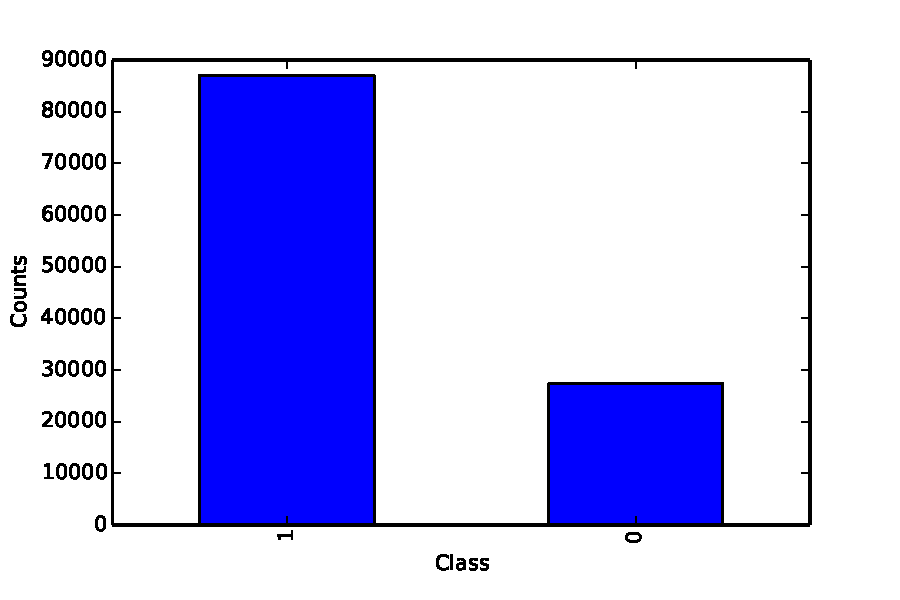
\includegraphics[width=5in, height=3in]{plot_de1.pdf}
% where an .eps filename suffix will be assumed under latex, 
% and a .pdf suffix will be assumed for pdflatex; or what has been declared
% via \DeclareGraphicsExtensions.
\caption{Class counts in training dataset.}
\label{fig_de1}
\end{figure}
Because of anonymization we do not know information about our features. Hence we are led to treat categorical features as nominal features, which creates problems for preprocessing that we will mention later. The number of distinct values in categorical features is shown in the table of figure [[2]].
%
%plot
%
Moreover our dataset contains a lot of missing values. 


\section{Preprocessing}
In the previous section were mentioned the types of variables which the given dataset consists of. Numerical values are in appropriate form to be processed by machine learning algorithms as most of the times they represent ordinal measures. On the other hand, categorical values need to be preprocessed and transformed into numerical so that the algorithms can be applied on them too. In addition, the project team had to overcome the obstacle of missing values in the dataset as they constituted a considerable percentile of the available data. Lastly, the standardization of all variable values was decided as the scale of values was different for every variable. 

\subsection{Categorical features conversion}
The preprocessing of features with categorical values is a process that the approach that is followed by the team can greatly influence the final outcome of the analysis. The most common and successful approach in this case is an implemented method called One-Hot-Encoder, which expands the dataset by as many new features as the possible values of every categorical feature, having zeros in new features if an observation does not have this categorical value or one in the new feature that corresponds to the value of this observation. This transformation creates a very sparse matrix.

Unfortunately, in our case this method could not applied because one of the categorical variables had 18,000 distinct values, so the application of such an approach would lead to a matrix with several thousands of features, and the final matrix would be extremely sparse. Additionally, the main problem would be that matrices with so large dimensions in features, as well as in observations need computers with much higher processing power than the conventional computers available to the members of the team, as the computational complexity increases exponentially.

As a result of the above observation, the team decided to deploy an alternative approach which was based on the idea of replacing each categorical value  a probability value. For every categorical distinct value of each variable we calculated the conditional probability on getting a response value of one when this categorical value appears, and fiannly replaced the categorical values with the corresponding conditional probability.
\subsection{Filling missing values}
\subsection{Standardization}
\subsection{Dimensionality reduction (PCA)}


\section{The Kaggle's winning solution}
Dexter’s Lab won this competition by applying intelligent approach to feature engineering.  The winning team's approach was that the most important task in feature engineering was to decode the anonymous variables. They successfully did some decoding related to dates and formulas like ‘data of observation’, ‘contract start date’ etc. One very important assumption they have made is that variable ‘v22’ is a customer and ‘v56/v113’ is the product type. Based on this assumption they have dropped v22 from the analysis.

The target value was very pushy for each ‘v22-Customer’, ‘v40/v50-Contract Start Data’ and resulted crediting target sequence through ‘lag target’ and ‘lead target’ variables. 

The winning team has used XGBoost model to achieve 0.42193 score and compared the results with other models like NNETS, linear SVM, Elastic Nets, XGBoost with count and regularized greedy forest which almost gave the same results.


\subsection{Subsection Heading Here}
Subsection text here.


\subsubsection{Subsubsection Heading Here}
Subsubsection text here.


% An example of a floating figure using the graphicx package.
% Note that \label must occur AFTER (or within) \caption.
% For figures, \caption should occur after the \includegraphics.
% Note that IEEEtran v1.7 and later has special internal code that
% is designed to preserve the operation of \label within \caption
% even when the captionsoff option is in effect. However, because
% of issues like this, it may be the safest practice to put all your
% \label just after \caption rather than within \caption{}.
%
% Reminder: the "draftcls" or "draftclsnofoot", not "draft", class
% option should be used if it is desired that the figures are to be
% displayed while in draft mode.
%
%\begin{figure}[!t]
%\centering
%\includegraphics[width=2.5in]{myfigure}
% where an .eps filename suffix will be assumed under latex, 
% and a .pdf suffix will be assumed for pdflatex; or what has been declared
% via \DeclareGraphicsExtensions.
%\caption{Simulation Results}
%\label{fig_sim}
%\end{figure}

% Note that IEEE typically puts floats only at the top, even when this
% results in a large percentage of a column being occupied by floats.


% An example of a double column floating figure using two subfigures.
% (The subfig.sty package must be loaded for this to work.)
% The subfigure \label commands are set within each subfloat command, the
% \label for the overall figure must come after \caption.
% \hfil must be used as a separator to get equal spacing.
% The subfigure.sty package works much the same way, except \subfigure is
% used instead of \subfloat.
%
%\begin{figure*}[!t]
%\centerline{\subfloat[Case I]\includegraphics[width=2.5in]{subfigcase1}%
%\label{fig_first_case}}
%\hfil
%\subfloat[Case II]{\includegraphics[width=2.5in]{subfigcase2}%
%\label{fig_second_case}}}
%\caption{Simulation results}
%\label{fig_sim}
%\end{figure*}
%
% Note that often IEEE papers with subfigures do not employ subfigure
% captions (using the optional argument to \subfloat), but instead will
% reference/describe all of them (a), (b), etc., within the main caption.


% An example of a floating table. Note that, for IEEE style tables, the 
% \caption command should come BEFORE the table. Table text will default to
% \footnotesize as IEEE normally uses this smaller font for tables.
% The \label must come after \caption as always.
%
%\begin{table}[!t]
%% increase table row spacing, adjust to taste
%\renewcommand{\arraystretch}{1.3}
% if using array.sty, it might be a good idea to tweak the value of
% \extrarowheight as needed to properly center the text within the cells
%\caption{An Example of a Table}
%\label{table_example}
%\centering
%% Some packages, such as MDW tools, offer better commands for making tables
%% than the plain LaTeX2e tabular which is used here.
%\begin{tabular}{|c||c|}
%\hline
%One & Two\\
%\hline
%Three & Four\\
%\hline
%\end{tabular}
%\end{table}



\section{Conclusion}
The conclusion goes here.




% conference papers do not normally have an appendix


% use section* for acknowledgement
\section*{Acknowledgment}


The authors would like to thank...





\begin{thebibliography}{99}
\bibitem{ml1} Phil Simon (March 18, 2013). \emph{Too Big to Ignore: The Business Case for Big Data.} Wiley. p. 89. ISBN 978-1-118-63817-0.
\bibitem{pb1} Kate Palmer (July 13, 2015)  \emph{Insurance cheats cost households £90 a year as bogus claims reach record high}\\
\url{http://www.telegraph.co.uk/journalists/kate-palmer/11736121/Insurance-cheats-cost-households-90-a-year-as-bogus-claims-reach-record-high.html}


\end{thebibliography}




\end{document}


